% Options for packages loaded elsewhere
% Options for packages loaded elsewhere
\PassOptionsToPackage{unicode}{hyperref}
\PassOptionsToPackage{hyphens}{url}
\PassOptionsToPackage{dvipsnames,svgnames,x11names}{xcolor}
%
\documentclass[
  letterpaper,
  DIV=11,
  numbers=noendperiod,
  oneside]{scrartcl}
\usepackage{xcolor}
\usepackage[left=1in,marginparwidth=2.0666666666667in,textwidth=4.1333333333333in,marginparsep=0.3in]{geometry}
\usepackage{amsmath,amssymb}
\setcounter{secnumdepth}{-\maxdimen} % remove section numbering
\usepackage{iftex}
\ifPDFTeX
  \usepackage[T1]{fontenc}
  \usepackage[utf8]{inputenc}
  \usepackage{textcomp} % provide euro and other symbols
\else % if luatex or xetex
  \usepackage{unicode-math} % this also loads fontspec
  \defaultfontfeatures{Scale=MatchLowercase}
  \defaultfontfeatures[\rmfamily]{Ligatures=TeX,Scale=1}
\fi
\usepackage{lmodern}
\ifPDFTeX\else
  % xetex/luatex font selection
\fi
% Use upquote if available, for straight quotes in verbatim environments
\IfFileExists{upquote.sty}{\usepackage{upquote}}{}
\IfFileExists{microtype.sty}{% use microtype if available
  \usepackage[]{microtype}
  \UseMicrotypeSet[protrusion]{basicmath} % disable protrusion for tt fonts
}{}
\makeatletter
\@ifundefined{KOMAClassName}{% if non-KOMA class
  \IfFileExists{parskip.sty}{%
    \usepackage{parskip}
  }{% else
    \setlength{\parindent}{0pt}
    \setlength{\parskip}{6pt plus 2pt minus 1pt}}
}{% if KOMA class
  \KOMAoptions{parskip=half}}
\makeatother
% Make \paragraph and \subparagraph free-standing
\makeatletter
\ifx\paragraph\undefined\else
  \let\oldparagraph\paragraph
  \renewcommand{\paragraph}{
    \@ifstar
      \xxxParagraphStar
      \xxxParagraphNoStar
  }
  \newcommand{\xxxParagraphStar}[1]{\oldparagraph*{#1}\mbox{}}
  \newcommand{\xxxParagraphNoStar}[1]{\oldparagraph{#1}\mbox{}}
\fi
\ifx\subparagraph\undefined\else
  \let\oldsubparagraph\subparagraph
  \renewcommand{\subparagraph}{
    \@ifstar
      \xxxSubParagraphStar
      \xxxSubParagraphNoStar
  }
  \newcommand{\xxxSubParagraphStar}[1]{\oldsubparagraph*{#1}\mbox{}}
  \newcommand{\xxxSubParagraphNoStar}[1]{\oldsubparagraph{#1}\mbox{}}
\fi
\makeatother


\usepackage{longtable,booktabs,array}
\usepackage{calc} % for calculating minipage widths
% Correct order of tables after \paragraph or \subparagraph
\usepackage{etoolbox}
\makeatletter
\patchcmd\longtable{\par}{\if@noskipsec\mbox{}\fi\par}{}{}
\makeatother
% Allow footnotes in longtable head/foot
\IfFileExists{footnotehyper.sty}{\usepackage{footnotehyper}}{\usepackage{footnote}}
\makesavenoteenv{longtable}
\usepackage{graphicx}
\makeatletter
\newsavebox\pandoc@box
\newcommand*\pandocbounded[1]{% scales image to fit in text height/width
  \sbox\pandoc@box{#1}%
  \Gscale@div\@tempa{\textheight}{\dimexpr\ht\pandoc@box+\dp\pandoc@box\relax}%
  \Gscale@div\@tempb{\linewidth}{\wd\pandoc@box}%
  \ifdim\@tempb\p@<\@tempa\p@\let\@tempa\@tempb\fi% select the smaller of both
  \ifdim\@tempa\p@<\p@\scalebox{\@tempa}{\usebox\pandoc@box}%
  \else\usebox{\pandoc@box}%
  \fi%
}
% Set default figure placement to htbp
\def\fps@figure{htbp}
\makeatother


% definitions for citeproc citations
\NewDocumentCommand\citeproctext{}{}
\NewDocumentCommand\citeproc{mm}{%
  \begingroup\def\citeproctext{#2}\cite{#1}\endgroup}
\makeatletter
 % allow citations to break across lines
 \let\@cite@ofmt\@firstofone
 % avoid brackets around text for \cite:
 \def\@biblabel#1{}
 \def\@cite#1#2{{#1\if@tempswa , #2\fi}}
\makeatother
\newlength{\cslhangindent}
\setlength{\cslhangindent}{1.5em}
\newlength{\csllabelwidth}
\setlength{\csllabelwidth}{3em}
\newenvironment{CSLReferences}[2] % #1 hanging-indent, #2 entry-spacing
 {\begin{list}{}{%
  \setlength{\itemindent}{0pt}
  \setlength{\leftmargin}{0pt}
  \setlength{\parsep}{0pt}
  % turn on hanging indent if param 1 is 1
  \ifodd #1
   \setlength{\leftmargin}{\cslhangindent}
   \setlength{\itemindent}{-1\cslhangindent}
  \fi
  % set entry spacing
  \setlength{\itemsep}{#2\baselineskip}}}
 {\end{list}}
\usepackage{calc}
\newcommand{\CSLBlock}[1]{\hfill\break\parbox[t]{\linewidth}{\strut\ignorespaces#1\strut}}
\newcommand{\CSLLeftMargin}[1]{\parbox[t]{\csllabelwidth}{\strut#1\strut}}
\newcommand{\CSLRightInline}[1]{\parbox[t]{\linewidth - \csllabelwidth}{\strut#1\strut}}
\newcommand{\CSLIndent}[1]{\hspace{\cslhangindent}#1}



\setlength{\emergencystretch}{3em} % prevent overfull lines

\providecommand{\tightlist}{%
  \setlength{\itemsep}{0pt}\setlength{\parskip}{0pt}}



 


\usepackage{amsfonts}
\usepackage{amsmath}
\usepackage{braket}
\KOMAoption{captions}{tableheading}
\makeatletter
\@ifpackageloaded{caption}{}{\usepackage{caption}}
\AtBeginDocument{%
\ifdefined\contentsname
  \renewcommand*\contentsname{Table of contents}
\else
  \newcommand\contentsname{Table of contents}
\fi
\ifdefined\listfigurename
  \renewcommand*\listfigurename{List of Figures}
\else
  \newcommand\listfigurename{List of Figures}
\fi
\ifdefined\listtablename
  \renewcommand*\listtablename{List of Tables}
\else
  \newcommand\listtablename{List of Tables}
\fi
\ifdefined\figurename
  \renewcommand*\figurename{Figure}
\else
  \newcommand\figurename{Figure}
\fi
\ifdefined\tablename
  \renewcommand*\tablename{Table}
\else
  \newcommand\tablename{Table}
\fi
}
\@ifpackageloaded{float}{}{\usepackage{float}}
\floatstyle{ruled}
\@ifundefined{c@chapter}{\newfloat{codelisting}{h}{lop}}{\newfloat{codelisting}{h}{lop}[chapter]}
\floatname{codelisting}{Listing}
\newcommand*\listoflistings{\listof{codelisting}{List of Listings}}
\makeatother
\makeatletter
\makeatother
\makeatletter
\@ifpackageloaded{caption}{}{\usepackage{caption}}
\@ifpackageloaded{subcaption}{}{\usepackage{subcaption}}
\makeatother
\makeatletter
\@ifpackageloaded{sidenotes}{}{\usepackage{sidenotes}}
\@ifpackageloaded{marginnote}{}{\usepackage{marginnote}}
\makeatother
\usepackage{bookmark}
\IfFileExists{xurl.sty}{\usepackage{xurl}}{} % add URL line breaks if available
\urlstyle{same}
\hypersetup{
  colorlinks=true,
  linkcolor={blue},
  filecolor={Maroon},
  citecolor={Blue},
  urlcolor={Blue},
  pdfcreator={LaTeX via pandoc}}


\author{}
\date{}
\begin{document}


\subsection{14/10/2026}\label{section}

Supervisor meeting:

\begin{itemize}
\item
  Dynamical map vs simulation plot atop on ech other to confirm
\item
  potential stretch goals:

  \begin{itemize}
  \tightlist
  \item
    different spectral function
  \item
    2 site impurity potentially
  \end{itemize}
\item
  TTM - plotting error more specifically
\item
  TTM - discretization error is less important than thought - TT is
  exact for its timestep which is what we're interestint
\item
  avoid non thermalizing bound states as a general rule (may be
  interesting as stretch goal)
\item
  wierdness for system energy near bounds of bath - non thermalization
\item
  presentation:

  \begin{itemize}
  \tightlist
  \item
    need to convey why is this question interesting
  \item
    don't need to overdo it; can keep it fairly conceptual
  \end{itemize}
\item
  try evolution which starts at thermalization - it may do some wierd
  stuff
\item
  recent paper which bites out semi circle - spectral function relation
  to memory; correlations in the bath - acquire later
\end{itemize}

To do:

\begin{itemize}
\tightlist
\item
  dynamical propagation vs simulation propagation plot - subtract em
  from each other to show they equal
\item
  Consider plotting simulation evolution that starts at thermalization
  occupancy
\item
  attempt TTM implementation - don't worry if it takes longer; switch to
  presentation otherwise

  \begin{itemize}
  \tightlist
  \item
    If it works quickly, plot it over a basic testing range of
    parameters
  \end{itemize}
\item
  Draft presentation:

  \begin{itemize}
  \tightlist
  \item
    Setup slides
  \item
    use slides to figure out what additional plots i'd like to generate
    for illustrative purposes
  \end{itemize}
\end{itemize}

\subsection{17/10/2026}\label{section-1}

Going to start on the presentation today. Copy/pasting the things i need
to include:

\begin{itemize}
\tightlist
\item
  Field background - memory effects in quantum thermodynamic systems
\item
  Project impetus - unclear and somewhat contradicting memory
  definitions for quantum non markovianity vs classical non markovianity
\item
  Project setup - simulation of star geometry system in order to produce
  dynamical maps which can be used to test different memory definitions
\item
  Work done thus far
\item
  Preliminary results
\item
  Future plans
\end{itemize}

Setting up slides as:

\begin{enumerate}
\def\labelenumi{\arabic{enumi}.}
\tightlist
\item
  Title slide
\item
  Field background

  \begin{itemize}
  \tightlist
  \item
    Quantum thermodynamics as a concept\hspace{0pt}
  \item
    Compare to classical thermodynamics -- recap concepts of system,
    bath, thermalization\hspace{0pt} - stochastics may also be worth
    mentioning
  \item
    Introduce classical ideas of memory effects/markovianity\hspace{0pt}
  \end{itemize}
\item
  Project motivation and background

  \begin{itemize}
  \tightlist
  \item
    State that memory effects in quantum systems aren't fully understood
  \item
    This project aims to compare different definitions of non
    markovianity by numerical simulation
  \item
    Name drop three definitions
  \item
    This is being done in order to provide additional research context
    to this area
  \end{itemize}
\item
  Project setup (model explanation)

  \begin{itemize}
  \tightlist
  \item
    introduce computational model:

    \begin{itemize}
    \tightlist
    \item
      1 dot system connected to a discreetized bath
    \item
      Note this discreetized bath is different to classical case where
      bath is assumed homogeneous
    \item
      Note spectral function as characterizing bath shape (plot may be
      useful here)
    \end{itemize}
  \item
    maybe show hamiltonian?
  \end{itemize}
\item
  Work done thus far part 1:

  \begin{itemize}
  \tightlist
  \item
    Build up simulation utility - use this as opportunity to explain how
    the simulation is being propagated through time
  \item
    Show initial simulation test data here (gif of bath/system
    occupation evolution may help show what this evolution looks like)
  \item
    maybe run an additional sim where the system starts at
    thermalization - show plot w/occupation start 0, 1, n\_\{thermal\}
    all in one plot - use this to highlight the wierdness of quantum
    memory effects
  \end{itemize}
\item
  Work done thus far part 2:

  \begin{itemize}
  \tightlist
  \item
    Build up dynamic map extraction - explain dynamic map is ``reduced''
    object which contains full dynamical information
  \item
    Show the simulation vs dynamic map evolution to show that this does
    indeed perfectly encapsulate the dynamics of the system
  \item
    State that this object is what will be analysed to extract memory
    definitions
  \end{itemize}
\item
  Future plans:

  \begin{itemize}
  \tightlist
  \item
    Implement memory definitions:

    \begin{itemize}
    \tightlist
    \item
      immediate next step: implement memory kernel definition as
      ``pathfinding'' def for formalism
    \item
      examine it's data to gain familiarity w/memory
    \end{itemize}
  \item
    Implement other memory definitions using the insight gained
  \item
    test the definitions against each other with the spectral function
    as the main ``experimental nob''
  \end{itemize}
\item
  Bibliography
\end{enumerate}

Given that, have quickly tested the initially thermalized occupation
setup, and it is indeed odd:

\begin{figure}

\centering{

\pandocbounded{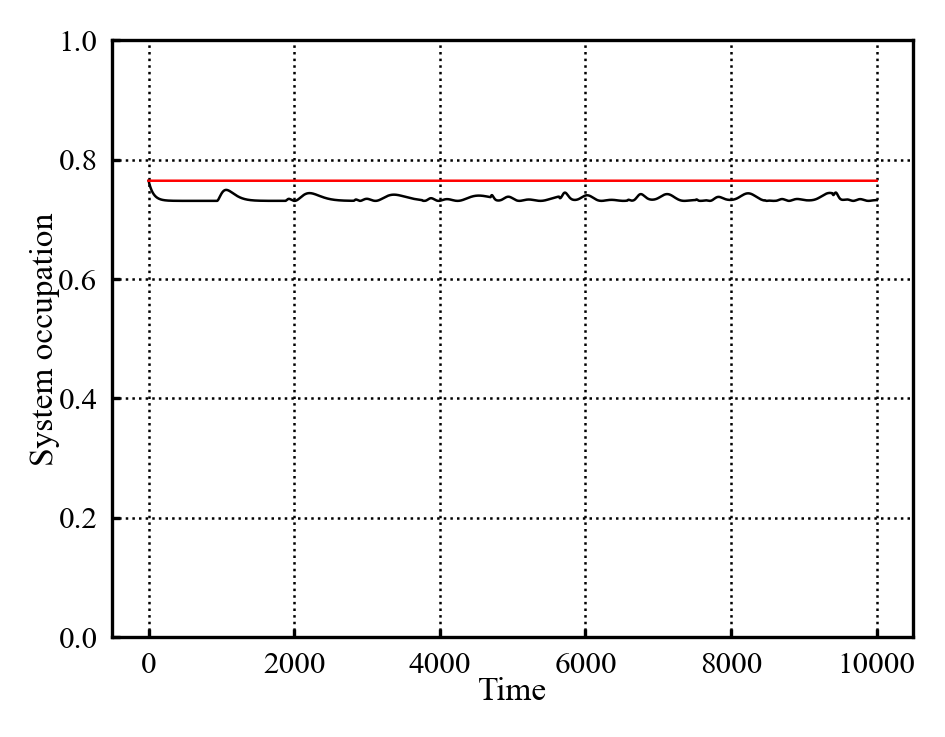
\includegraphics[keepaspectratio]{figures/simFromThermalization_systemOccupation.png}}

}

\caption{\label{fig-thermalInitialOcc}System evolution for
\(n_{sys}(0)=\lim_{t\to\infty}n_{sys}(t)\)}

\end{figure}%

Which is what was expected; good to see that it behaves interstingly.

Also looking to generate gif versions of some of the plots for
presentation reasons using (\textbf{pltGifs?}), (Daniel 2018). Have
fiddled a bunch and produced the following:

\url{animated_systenBathEvo.mp4}

which quarto doesn't seem to be rendering\ldots{} tmr problem.

\subsection{18/10/2026}\label{section-2}

Fiddled a bit more w/animation plotting to give better control over
animation length. Am having issues displaying these on quarto;
attempting to troubleshoot. Can't display local mp4 or gif, however can
display yt vid. Its fine\ldots{} Spent some time quickly tidying up the
simulation queue code - packed sim args into a dictionary to make
variations and ``standard sets'' easier. Have also built some additional
utilities to make running datasets and such easier.

Am trying to reproduce these Figure~\ref{fig-thermalInitialOcc} results
after cleaning up the code, however can't. I suspect i made a coding
error when producing this plot and accidentally added a small value to
the analytical thermalization. Figure~\ref{fig-thermalInitialOcc} seems
to thermalize to a\(n\approx 0.73\) in this plot (before recurrence due
to model finite size occurs). As such, i think this plot is wrong and to
be disregarded.

Have produced plot of dynamic vs simulated evolution:

\begin{figure}

\centering{

\pandocbounded{\includegraphics[keepaspectratio]{figures/standardDualSim_compareEvo.png}}

}

\caption{\label{fig-dualVsSim}System evolution propagated by dynamic map
and simulation}

\end{figure}%

As well as adding some utilities to make using the dual sim system
easier.

Have produced animated gif illustration of star geometry setup for the
dissertation presentation.

\subsection{19/10/2026}\label{section-3}

Am thinking in terms of what background/theoretical content needs to be
included. It'd be good to include the names/equations for the different
non markovianity defs.

(Rivas and Huelga 2012) includes explanation of memory kernels.

(Milz and Modi 2021) may also be a good resource; it includes classical
non markovianity which will be a useful reference point for presentation
reasons.

\subsubsection{Reading notes (Milz and Modi
2021)}\label{reading-notes-quantumstochasticprocesses2021}

This is a long review paper. Introduction helps motivate the topic. Open
systems are ones connected to some external environment that cannot be
modelled for computational reasons. Stochastics aims to treat these
environmental interactions statistically in order to model the system.
Practical interest for range of reasons:

\begin{itemize}
\tightlist
\item
  better understanding of environmental interaction will help create
  fault tolerant qubits for quantum computing reasons
\item
  Modelling many body quantum systems, with applications across
  condensed matter physics, quantum chemistry\ldots{}
\end{itemize}

This review aims to introduce and explain memory effects in quantum
stochastic processes, and relate them to classical stochastic theories.

Section 2 of the paper outlines classical examples; this will likely be
quite useful for presentation reasons. Uses the example of sequential
random dice tosses in order to illustrate stochastic processes. Uses
this to illustrate memory effects - probability \(P_{n}(O)\) does not
depend on previous outcomes for memoryless systems. ``Memoryless''
Markov processes are introduced.

\marginnote{\begin{footnotesize}

The dice example may be a good example to use; i wonder if a random walk
could help illustrate a non markovian process visually. Paper uses
examples of poorly retossed dice instead to illustrate conditional
probability on past events.

\end{footnotesize}}

This paper looks quite interesting and worth going into greater depth
later; for now however am just going to extract things useful for
presentation. The poorly tossed dice example is probably useful way of
illustrating memory effects; although i do wonder if a random walk may
be better.

Quickly checking through the rest of the paper, it does discuss the
complete-positivity memory definition.

\subsubsection{presentation work
continued}\label{presentation-work-continued}

(Breuer, Laine, and Piilo 2009) is seemingly the original paper
discussing information backflow. Therefore for the 3 measures mentioned,
i think i can cite them from:

\begin{itemize}
\tightlist
\item
  memory kernels (Rivas and Huelga 2012)
\item
  Information backflow (Breuer, Laine, and Piilo 2009)
\item
  Failure of complete positivity (Milz and Modi 2021)
\end{itemize}

Thats reassuring. Have produced a diagram to illustrate open vs closed
systems. I think the best way to illustrate that is unfortunately
showing the conditional probability expression for a set of sequential
events w/memory. I'd rather do it diagramatically, however am unsure
there is a good way to do so\ldots{} Might be able to do it as a table
of outcomes over time steps; one column represents a memoryless system,
the other a memory-full system - can then show memory effects timestep
by timestep using a concrete example.

Have ignored that for now and gotten most of the rest of the
presentation drafted.

Have got a full draft (minus the references which can be added later)
here:
\href{https://uob-my.sharepoint.com/:p:/g/personal/hx21918_bristol_ac_uk/IQAxHoGUDOXaQ5f2EMPY8mX0ATvUz0yuHUQQV01cOwx3EG4?e=jM7VKp}{presentation
draft}.

Things that still need doing:

\begin{itemize}
\tightlist
\item
  Equations are blurry; this may be due to settings in libreoffice tex
  processor
\item
  Fix system gif on slide 4 - in presenter mode it overlaps the plot
\item
  check w/supervisors that this is what i need
\item
  add references
\end{itemize}

\phantomsection\label{refs}
\begin{CSLReferences}{1}{0}
\bibitem[\citeproctext]{ref-MeasureForNonMarkovianity2009}
Breuer, Heinz-Peter, Elsi-Mari Laine, and Jyrki Piilo. 2009. {``Measure
for the {Degree} of {Non}-{Markovian} {Behavior} of {Quantum}
{Processes} in {Open} {Systems}.''} \emph{Physical Review Letters} 103
(21): 210401. \url{https://doi.org/10.1103/PhysRevLett.103.210401}.

\bibitem[\citeproctext]{ref-pltAnimationHelp}
Daniel. 2018. {``Python {Matplotlib} {FuncAnimation} + {Saving}.''}
Forum post. \emph{Stack Overflow}.
\url{https://stackoverflow.com/q/49133207}.

\bibitem[\citeproctext]{ref-QuantumStochasticProcesses2021}
Milz, Simon, and Kavan Modi. 2021. {``Quantum {Stochastic} {Processes}
and {Quantum} Non-{Markovian} {Phenomena} {\textbar} {PRX} {Quantum}.''}
\url{https://doi.org/10.1103/PRXQuantum.2.030201}.

\bibitem[\citeproctext]{ref-OpenQuantumSystemsIntro2012}
Rivas, Ángel, and Susana F Huelga. 2012. \emph{Open {Quantum} {Systems}.
{An} {Introduction}}.
https://doi.org/\url{https://doi.org/10.48550/arXiv.1104.5242}.

\end{CSLReferences}




\end{document}
